\documentclass[12pt, letterpaper]{article}
\usepackage[margin=1in]{geometry}
\usepackage[T1]{fontenc}
\usepackage{lmodern}
\usepackage{cmap}
\usepackage[utf8]{inputenc}
\usepackage{amsmath, amssymb, amsthm}
\usepackage{mathtools}
\usepackage{enumitem}
\usepackage{booktabs}
\usepackage{xcolor}
\usepackage{titlesec}
\usepackage{parskip}
\usepackage{hyperref}
\usepackage{fancyhdr}
\usepackage{tcolorbox}
\usepackage{graphicx}
\usepackage{caption}
\tcbuselibrary{skins, breakable}

\definecolor{darkblue}{RGB}{15,55,115}
\definecolor{midblue}{RGB}{30,100,180}
\definecolor{theorybg}{RGB}{245,250,255}
\definecolor{questionbg}{RGB}{255,252,240}
\definecolor{evencolor}{RGB}{60,0,100}

\hypersetup{colorlinks=true,linkcolor=darkblue,urlcolor=midblue,
  pdftitle={Ljungqvist \& Sargent --- Recursive Macroeconomic Theory --- Complete Solutions, Chapter 5}}

\setlength{\headheight}{14pt}
\pagestyle{fancy}
\fancyhf{}
\renewcommand{\headrulewidth}{0.4pt}
\fancyhead[L]{\small\textcolor{darkblue}{\textit{Ljungqvist \& Sargent --- Recursive Macroeconomic Theory}}}
\fancyhead[R]{\small\textcolor{darkblue}{\thepage}}
\fancyfoot[C]{\small\textcolor{gray}{Complete Solutions --- Chapter 5}}

\titleformat{\section}[block]
  {\large\bfseries\color{darkblue}}{}{0pt}{}
  [\vspace{2pt}\color{darkblue}\rule{\textwidth}{1.5pt}\vspace{4pt}]

\titleformat{\subsection}[block]
  {\normalsize\bfseries\color{midblue}}{}{0pt}{}
  [\vspace{1pt}\color{midblue}\rule{0.5\textwidth}{0.8pt}\vspace{3pt}]

\tcbset{
  theorybox/.style={
    enhanced,breakable,colback=theorybg,colframe=darkblue,
    fonttitle=\bfseries\small, coltitle=white,boxrule=0.5pt,arc=3pt,
    left=6pt,right=6pt,top=4pt,bottom=4pt,title={Key Theory},
  },
  questionbox/.style={
    enhanced,breakable,colback=questionbg,colframe=gray!60,
    fonttitle=\bfseries\small\color{gray!60!black},boxrule=0.4pt,arc=2pt,
    left=6pt,right=6pt,top=4pt,bottom=4pt,title={\textit{Question}},
  },
  oddbox/.style={
    enhanced,breakable,colback=white,colframe=darkblue,
    attach boxed title to top left={yshift=-2mm,xshift=6mm},
    boxed title style={colback=darkblue,colframe=darkblue,arc=2pt,
      boxrule=0pt,left=6pt,right=6pt,top=3pt,bottom=3pt},
    fonttitle=\bfseries\large\color{white},
    boxrule=0.8pt,arc=3pt,
    left=8pt,right=8pt,top=10pt,bottom=6pt,
  },
  evenbox/.style={
    enhanced,breakable,colback=white,colframe=evencolor,
    attach boxed title to top left={yshift=-2mm,xshift=6mm},
    boxed title style={colback=evencolor,colframe=evencolor,arc=2pt,
      boxrule=0pt,left=6pt,right=6pt,top=3pt,bottom=3pt},
    fonttitle=\bfseries\large\color{white},
    boxrule=0.8pt,arc=3pt,
    left=8pt,right=8pt,top=10pt,bottom=6pt,
  },
  databox/.style={
    enhanced,breakable,colback=gray!8,colframe=gray!55,
    fonttitle=\bfseries\small\color{gray!60!black},boxrule=0.4pt,arc=2pt,
    left=6pt,right=6pt,top=4pt,bottom=4pt,title={Numerical exercise --- see the companion code},
  },
  trapbox/.style={
    enhanced,breakable,colback=red!4,colframe=red!45!black,
    fonttitle=\bfseries\small\color{white},boxrule=0.4pt,arc=2pt,
    coltitle=white,
    left=6pt,right=6pt,top=4pt,bottom=4pt,title={Where this goes wrong},
  },
}

\newcommand{\pd}[2]{\dfrac{\partial #1}{\partial #2}}
\newcommand{\dd}[2]{\dfrac{d #1}{d #2}}
\newcommand{\MRS}{\mathrm{MRS}}
\newcommand{\MRT}{\mathrm{MRT}}
\newcommand{\MU}{\mathrm{MU}}
\newcommand{\Var}{\mathrm{Var}}
\newcommand{\Cov}{\mathrm{Cov}}
\newcommand{\E}{\mathrm{E}}
\newcommand{\MPK}{\mathrm{MPK}}
\newcommand{\MPL}{\mathrm{MPL}}
\newcommand{\stst}{^{\ast}}

\setlist[enumerate,1]{label=(\alph*),itemsep=6pt,parsep=2pt}
\setlist[enumerate,2]{label=(\roman*),itemsep=3pt}


\newcommand{\tr}{\operatorname{trace}}

\begin{document}

%======================================================================
% TITLE PAGE
%======================================================================
\begin{titlepage}
\centering
\vspace*{2.5cm}
{\Huge\bfseries\color{darkblue} Recursive Macroeconomic Theory\par}
\vspace{6pt}
{\large Lars Ljungqvist \& Thomas J. Sargent (4th ed., 2018)\par}
\vspace{1.4cm}
{\LARGE\bfseries Complete Solutions\par}
\vspace{6pt}
{\LARGE\bfseries Chapter 5 --- Linear Quadratic Dynamic Programming\par}
\vspace{1.2cm}
{\large All 14 end-of-chapter exercises, 5.1--5.14 (pp.~145--155)\par}
\vspace{2cm}

\begin{tcolorbox}[theorybox,title={What is in this file},width=0.86\textwidth]
\small
Every exercise is mapped into the book's regulator,
$\max -\sum_t\beta^t\{x_t'Rx_t+u_t'Qu_t+2u_t'Hx_t\}$ s.t.\ $x_{t+1}=Ax_t+Bu_t+C\epsilon_{t+1}$,
whose solution is $v(x)=-x'Px-d$, $u=-Fx$. The analytical parts (derivations, closed forms,
existence conditions, estimation strategies) are done by hand; numerical parts use the program of
Exercise~5.1(b), written in Python instead of Matlab.

\smallskip
The companion notebook \texttt{ls\_ch05.ipynb} (same folder) computes every number quoted here and
checks each one by an independent route with an \texttt{assert}: Riccati iteration vs
\texttt{scipy.linalg.solve\_discrete\_are} vs Howard policy iteration; closed forms vs the LQ
solution; Lyapunov solutions vs Monte Carlo; Kalman log-likelihood vs the direct Gaussian density.

\smallskip
Question boxes give a condensed statement and the page; see the book for the full text. Where the
book gives no parameter values we state the ones used. Blue boxes are odd-numbered exercises,
purple boxes even-numbered ones.
\end{tcolorbox}

\vfill
{\small MPE Insper --- Macroeconomia I --- 2026, 3\textordmasculine{} trimestre\par}
\end{titlepage}

\tableofcontents
\newpage

%======================================================================
\section{Chapter 5 \quad Linear Quadratic Dynamic Programming}
%======================================================================

\begin{tcolorbox}[theorybox,title={Chapter 5 Overview}]
\textbf{Regulator.} Maximise $-E_0\sum_t\beta^t\{x_t'Rx_t+u_t'Qu_t\}$ s.t.\
$x_{t+1}=Ax_t+Bu_t+C\epsilon_{t+1}$, $E\epsilon\epsilon'=I$ (5.3.1)--(5.3.3). The value is
$v(x)=-x'Px-d$ (5.3.4) with
\begin{gather*}
P=R+\beta A'PA-\beta^2A'PB(Q+\beta B'PB)^{-1}B'PA,\\
F=\beta(Q+\beta B'PB)^{-1}B'PA,\qquad d=\frac{\beta}{1-\beta}\tr(PCC').
\end{gather*}
\textbf{Three ways to get $P$.} (i) Iterate the Riccati difference equation (5.2.9) from $P_0=0$;
(ii) Howard's policy iteration (5.2.10)--(5.2.11); (iii) the stable-invariant-subspace formula
$P=V_{21}V_{11}^{-1}$ of section 5.5 (what \texttt{scipy}'s DARE solver implements).

\textbf{Certainty equivalence.} $F$ does not depend on $C$; the noise only enters $d$.

\textbf{Two warnings that run through the exercises.} (a) Discounting is absorbed by
$\sqrt\beta A,\sqrt\beta B$: the relevant stability condition is that the eigenvalues of $A-BF$ be
below $1/\sqrt\beta$ in modulus. (b) When the return has a bliss point that can be reached forever by
borrowing (5.8, 5.10, 5.13(d)), the Riccati iteration from $P_0=0$ converges to $P=0$ --- a Ponzi
scheme --- while the \emph{stabilising} solution is the economically relevant one. Selecting it is
the regulator's way of imposing a no-Ponzi condition.

\textbf{Kalman filter} (5.6.2)--(5.6.3): $K=A\Sigma G'(G\Sigma G'+R)^{-1}$,
$\Sigma'=A\Sigma A'+CC'-K(G\Sigma G'+R)K'$; innovations $a_t=y_t-G\hat x_t$ with covariance
$G\Sigma G'+R$ (5.6.5).
\end{tcolorbox}

%----------------------------------------------------------------------
\subsection{The Riccati Equation and Howard's Algorithm}
%----------------------------------------------------------------------

%------- 5.1 -------
\begin{tcolorbox}[oddbox,title={Exercise 5.1 \quad Riccati equation with a cross-product term}]
\begin{tcolorbox}[questionbox]
p.~145. Maximise $-\sum_t\beta^t\{x_t'Rx_t+u_t'Qu_t+2u_t'Hx_t\}$ s.t.\ $x_{t+1}=Ax_t+Bu_t$.
(a) Show $u_t=-(Q+\beta B'PB)^{-1}(\beta B'PA+H)x_t$ with $P$ solving
$P=R+\beta A'PA-(\beta A'PB+H')(Q+\beta B'PB)^{-1}(\beta B'PA+H)$ \;(1).
(b) Write a program that solves (1) by iterating from $P=0$.
\end{tcolorbox}

\textbf{Solution:}

\textbf{(a)} Guess $V(x)=-x'Px$, $P$ symmetric. The Bellman equation is
\[
-x'Px=\max_u\big\{-x'Rx-u'Qu-2u'Hx-\beta(Ax+Bu)'P(Ax+Bu)\big\}.
\]
Expand the last term: $(Ax+Bu)'P(Ax+Bu)=x'A'PAx+2u'B'PAx+u'B'PBu$. The right side is
\[
-\big[x'(R+\beta A'PA)x+u'(Q+\beta B'PB)u+2u'(H+\beta B'PA)x\big].
\]
It is strictly concave in $u$ when $Q+\beta B'PB$ is positive definite (true since $Q>0$, $P\ge0$).
Using $\partial(u'Mu)/\partial u=2Mu$ for symmetric $M$ and $\partial(u'Nx)/\partial u=Nx$, the
first-order condition is
\[
-2(Q+\beta B'PB)u-2(\beta B'PA+H)x=0,
\]
so
\[
\boxed{u=-Fx,\qquad F=(Q+\beta B'PB)^{-1}(\beta B'PA+H).}
\]
Write $\mathcal Q\equiv Q+\beta B'PB$ and $\mathcal G\equiv\beta B'PA+H$, so $\mathcal QF=\mathcal G$.
At $u=-Fx$:
\[
u'\mathcal Qu=x'F'\mathcal QFx=x'\mathcal G'\mathcal Q^{-1}\mathcal Gx,\qquad
2u'\mathcal Gx=-2x'F'\mathcal Gx=-2x'\mathcal G'\mathcal Q^{-1}\mathcal Gx .
\]
Their sum is $-x'\mathcal G'\mathcal Q^{-1}\mathcal Gx$. The Bellman equation becomes
$x'Px=x'(R+\beta A'PA)x-x'\mathcal G'\mathcal Q^{-1}\mathcal Gx$ for all $x$; equating the
(symmetric) matrices,
\[
\boxed{P=R+\beta A'PA-(\beta A'PB+H')(Q+\beta B'PB)^{-1}(\beta B'PA+H),}
\]
which is (1), since $\mathcal G'=\beta A'PB+H'$. With $H=0$ it reduces to the book's (5.2.9) fixed
point and $F=\beta(Q+\beta B'PB)^{-1}B'PA$ (5.3.6). \checkmark

\emph{Condition.} For the problem to be concave jointly in $(x,u)$ we need
$\begin{bmatrix}R&H'\\H&Q\end{bmatrix}\ge0$, not only $R,Q>0$ separately.

\emph{A second route: remove the cross term.} Put $\tilde u=u+Q^{-1}Hx$. Then
$u'Qu+2u'Hx=\tilde u'Q\tilde u-x'H'Q^{-1}Hx$ and $Ax+Bu=(A-BQ^{-1}H)x+B\tilde u$. This is a
standard regulator with $\tilde R=R-H'Q^{-1}H$, $\tilde A=A-BQ^{-1}H$; its solution $\tilde F$ gives
$F=\tilde F+Q^{-1}H$. The notebook checks that both routes give the same $(P,F)$.

\textbf{(b)} The program (\texttt{olrp} in the notebook) sets $P_0=0$ and iterates
\[
P_{j+1}=R+\beta A'P_jA-(\beta A'P_jB+H')(Q+\beta B'P_jB)^{-1}(\beta B'P_jA+H)
\]
until $\max|P_{j+1}-P_j|<10^{-12}\max(1,\max|P_{j+1}|)$, then returns $P$ and $F$. $P_j$ is the
value matrix of the $j$-period problem with zero terminal value.

\begin{tcolorbox}[databox]
On five random problems ($n=4$, $k=2$, $\beta=.9$, joint return matrix positive definite) the
iteration converges in 17--74 steps and agrees with \texttt{scipy}'s DARE (called with
$\sqrt\beta A,\sqrt\beta B$ and $S=H'$) and with the cross-term-free transform to $5\times10^{-11}$; a
numerical maximisation of the Bellman right side returns $u=-Fx$.
\end{tcolorbox}
\end{tcolorbox}

%------- 5.2 -------
\begin{tcolorbox}[evenbox,title={Exercise 5.2 \quad (5.2.10)--(5.2.11) are the policy improvement algorithm}]
\begin{tcolorbox}[questionbox]
p.~145. Verify that $P_j=R+F_j'QF_j+\beta(A-BF_j)'P_j(A-BF_j)$ (5.2.10) and
$F_{j+1}=\beta(Q+\beta B'P_jB)^{-1}B'P_jA$ (5.2.11) implement the policy improvement algorithm for the
discounted regulator.
\end{tcolorbox}

\textbf{Solution:} Howard's algorithm (chapter 3) has two steps: \emph{evaluate} the current
policy forever, then \emph{improve} it by a one-step maximisation against that value.

\textbf{(5.2.10) is policy evaluation.} Under $u_t=-F_jx_t$ the state obeys
$x_{t+1}=(A-BF_j)x_t$, so $x_t=(A-BF_j)^tx_0$ and the period return is
$x_t'Rx_t+x_t'F_j'QF_jx_t=x_t'(R+F_j'QF_j)x_t$. The value of following $F_j$ forever is
\[
V_j(x_0)=-\sum_{t\ge0}\beta^tx_0'(A-BF_j)'^t(R+F_j'QF_j)(A-BF_j)^tx_0\equiv-x_0'P_jx_0,
\]
with $P_j$ the series displayed on p.~132 (it converges iff the eigenvalues of $A-BF_j$ are below
$1/\sqrt\beta$ in modulus). Split off $t=0$ and factor $(A-BF_j)$ out of the rest:
\begin{align*}
P_j&=(R+F_j'QF_j)+\beta(A-BF_j)'\Big[\sum_{t\ge0}\beta^t(A-BF_j)'^t(R+F_j'QF_j)(A-BF_j)^t\Big](A-BF_j)\\
&=R+F_j'QF_j+\beta(A-BF_j)'P_j(A-BF_j),
\end{align*}
which is (5.2.10): the value $V_j(x)=-x'Rx-x'F_j'QF_jx+\beta V_j[(A-BF_j)x]$.

\textbf{(5.2.11) is policy improvement.} Choose today's $u$ optimally, then follow $F_j$ from
tomorrow on:
$\max_u\{-x'Rx-u'Qu-\beta(Ax+Bu)'P_j(Ax+Bu)\}$. This is Exercise~5.1 with $H=0$ and $P=P_j$ held
fixed; its first-order condition $(Q+\beta B'P_jB)u=-\beta B'P_jAx$ gives
$u=-F_{j+1}x$ with $F_{j+1}=\beta(Q+\beta B'P_jB)^{-1}B'P_jA$, which is (5.2.11).

\textbf{The iteration improves and stops at the optimum.} Let $T_F$ be the evaluation operator
$T_Fv(x)=-x'(R+F'QF)x+\beta v[(A-BF)x]$ and $T$ the Bellman operator. By construction of $F_{j+1}$,
$T_{F_{j+1}}V_j=TV_j\ge T_{F_j}V_j=V_j$. $T_{F_{j+1}}$ is monotone, so applying it repeatedly,
$V_j\le T_{F_{j+1}}V_j\le T^2_{F_{j+1}}V_j\le\cdots\to V_{j+1}$: hence $V_{j+1}\ge V_j$, i.e.\
$P_{j+1}\le P_j$ in the positive-semidefinite order. If $F_{j+1}=F_j\equiv F$, substitute
$(Q+\beta B'PB)F=\beta B'PA$ into (5.2.10):
\begin{align*}
P&=R+F'QF+\beta A'PA-\beta A'PBF-\beta F'B'PA+\beta F'B'PBF\\
&=R+\beta A'PA+F'(Q+\beta B'PB)F-\beta A'PBF-\beta F'B'PA\\
&=R+\beta A'PA+\beta F'B'PA-\beta A'PBF-\beta F'B'PA
 =R+\beta A'PA-\beta A'PBF\\
&=R+\beta A'PA-\beta^2A'PB(Q+\beta B'PB)^{-1}B'PA,
\end{align*}
the algebraic Riccati equation of (5.2.9). So a fixed point of (5.2.10)--(5.2.11) solves the
Bellman equation. \hfill$\blacksquare$

\begin{tcolorbox}[databox]
On the problem of Exercise 5.3, from the (stable) initial rule ``invest half of income'', Howard's
algorithm needs \textbf{2} improvements to reach $F$ to $10^{-12}$ (the second only confirms);
the Riccati iteration from $P_0=0$ needs \textbf{496} steps. The notebook checks that (5.2.10)
equals the truncated series and a simulated discounted sum, that $P_j-P_{j+1}$ is positive
semidefinite at every step, and that the limit equals the DARE solution.
\end{tcolorbox}

\begin{center}
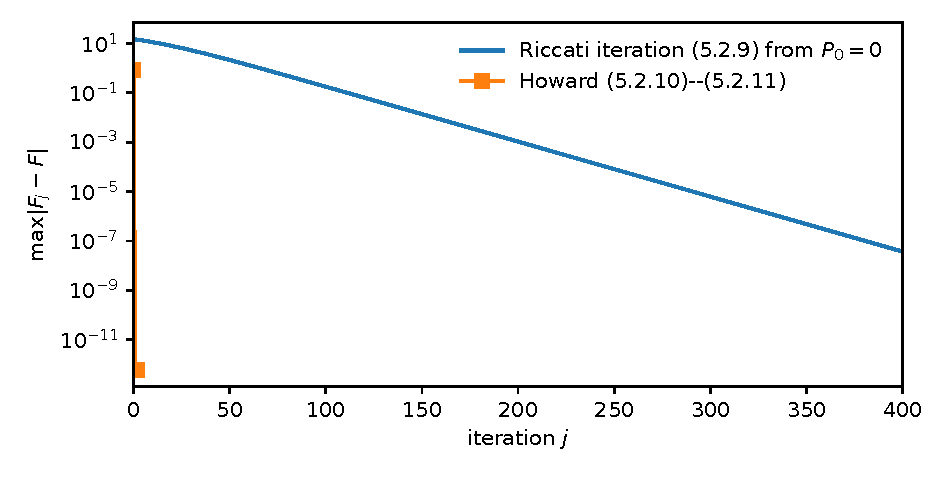
\includegraphics[width=0.85\linewidth]{fig/ls05_riccati_vs_howard.pdf}\\[3pt]
\captionof{figure}{Exercises 5.1--5.2. Distance of the policy to the optimum by iteration, problem of
Exercise 5.3. Howard's algorithm is Newton's method on the Riccati equation (quadratic convergence);
the Riccati iteration converges linearly at a rate set by the slowest closed-loop root.}
\end{center}
\end{tcolorbox}

%----------------------------------------------------------------------
\subsection{Household Problems as Regulators}
%----------------------------------------------------------------------

%------- 5.3 -------
\begin{tcolorbox}[oddbox,title={Exercise 5.3 \quad Saving with an adjustment cost on investment}]
\begin{tcolorbox}[questionbox]
pp.~145--146. Maximise $-\sum_t\beta^t\{(c_t-b)^2+\gamma i_t^2\}$ s.t.\ $c_t+i_t=ra_t+y_t$,
$a_{t+1}=a_t+i_t$, $y_{t+1}=\rho_1y_t+\rho_2y_{t-1}$. (a) Map into a linear regulator.
(b) Compute the policy for $[\beta,1+r,b,\gamma,\rho_1,\rho_2]=[.95,.95^{-1},30,1,1.2,-.3]$.
\end{tcolorbox}

\textbf{Solution:}

\textbf{(a)} State $x_t=[a_t,\ y_t,\ y_{t-1},\ 1]'$ (the constant carries the bliss point $b$),
control $u_t=i_t$. Using the budget, $c_t-b=ra_t+y_t-b-i_t=Sx_t-u_t$ with $S=[r,\ 1,\ 0,\ -b]$. Then
\[
(c_t-b)^2+\gamma i_t^2=(Sx_t-u_t)^2+\gamma u_t^2=x_t'S'Sx_t+(1+\gamma)u_t^2-2u_tSx_t,
\]
so $R=S'S$, $Q=1+\gamma$, $H=-S$ --- a cross term, hence the formulas of Exercise~5.1. The law of
motion is $x_{t+1}=Ax_t+Bu_t$ with
\[
A=\begin{bmatrix}1&0&0&0\\0&\rho_1&\rho_2&0\\0&1&0&0\\0&0&0&1\end{bmatrix},\qquad
B=\begin{bmatrix}1\\0\\0\\0\end{bmatrix}.
\]
$\begin{bmatrix}R&H'\\H&Q\end{bmatrix}=\begin{bmatrix}S'S&-S'\\-S&1+\gamma\end{bmatrix}\ge0$, so the
problem is concave. Roots of $1-1.2z+.3z^2$: $z=2.816,\ 1.184$, outside the unit circle, as assumed.

\textbf{(b)} With $r=.95^{-1}-1=0.05263$, the program of 5.1(b) gives
\[
\boxed{i_t=0.31671\,y_t+0.05589\,y_{t-1},\qquad c_t=0.05263\,a_t+0.68329\,y_t-0.05589\,y_{t-1}.}
\]
Closed-loop eigenvalues: $1,1,0.845,0.355$ (the unit roots are the constant and assets).

\emph{Reading the rule.} Neither $a_t$ nor $b$ enters investment. The Euler equation explains
both: raising $i_t$ by one unit and lowering $i_{t+1}$ by one leaves $a_{t+2}$ unchanged, lowers
$c_t$ by 1 and raises $c_{t+1}$ by $1+r$. Optimality requires
\[
(c_t-b)-\gamma i_t=\beta\big[(1+r)(c_{t+1}-b)-\gamma i_{t+1}\big].
\]
With $\beta(1+r)=1$ the $b$'s cancel, $c_t-\gamma i_t=c_{t+1}-\beta\gamma i_{t+1}$, so the bliss
point is irrelevant; and the household consumes the interest $ra_t$ on its assets, leaving the
investment decision to depend on the income process only. The notebook verifies this Euler equation
along a simulated path (residual $3\times10^{-11}$) and the rule by DARE.
\end{tcolorbox}

%------- 5.4 -------
\begin{tcolorbox}[evenbox,title={Exercise 5.4 \quad Durable goods and habit persistence}]
\begin{tcolorbox}[questionbox]
p.~146. As in 5.3 but with loss $(s_t-b)^2+\gamma i_t^2$, $s_t=\lambda h_t+\pi c_t$,
$h_{t+1}=\delta h_t+\theta c_t$. (a) Map into a regulator. (b) Policy for
$(\lambda,\pi,\delta,\theta)=(1,.05,.95,1)$; (c) for $(-1,1,.95,1)$; (d) interpret (b) as durables
and (c) as habits.
\end{tcolorbox}

\textbf{Solution:}

\textbf{(a)} Add $h_t$ to the state: $x_t=[a_t,\ y_t,\ y_{t-1},\ h_t,\ 1]'$, $u_t=i_t$. Substituting
$c_t=ra_t+y_t-i_t$:
\begin{align*}
s_t-b&=\lambda h_t+\pi(ra_t+y_t-i_t)-b=Sx_t-\pi u_t,\qquad S=[\pi r,\ \pi,\ 0,\ \lambda,\ -b],\\
h_{t+1}&=\theta r\,a_t+\theta y_t+\delta h_t-\theta u_t .
\end{align*}
Then $(s_t-b)^2+\gamma i_t^2=x_t'S'Sx_t+(\pi^2+\gamma)u_t^2-2\pi u_tSx_t$: $R=S'S$,
$Q=\pi^2+\gamma$, $H=-\pi S$, and
\[
A=\begin{bmatrix}1&0&0&0&0\\0&\rho_1&\rho_2&0&0\\0&1&0&0&0\\\theta r&\theta&0&\delta&0\\0&0&0&0&1\end{bmatrix},\qquad
B=\begin{bmatrix}1\\0\\0\\-\theta\\0\end{bmatrix}.
\]

\textbf{(b)--(c)} Same $(\beta,r,b,\gamma,\rho_1,\rho_2)$ as 5.3. Writing the rules for
consumption ($c=ra+y-i$):
\begin{align*}
\text{(b) durables:}\quad c_t&=0.35174\,a_t+2.52050\,y_t-0.61213\,y_{t-1}-0.28416\,h_t,\\
\text{(c) habits:}\quad c_t&=0.23180\,a_t+1.68809\,y_t-0.42542\,y_{t-1}-0.17021\,h_t,
\end{align*}
(investment $i_t=ra_t+y_t-c_t$). Closed-loop eigenvalues: (b) $1,1,0.845,0.367,0.355$;
(c) $1,1,0.845,0.601,0.355$. Riccati iteration, DARE and Howard agree to $10^{-7}$.

\textbf{(d)} In (b), $s_t=h_t+.05c_t$ and $h_{t+1}=.95h_t+c_t$: $c_t$ is \emph{purchases} of a
durable that depreciates at 5\%, and services come mostly from the stock. Buying is a way of saving:
a unit income shock raises purchases by 2.5 on impact (Figure~\ref{fig:dur}), a burst that builds the
stock, after which purchases fall back to the permanent-income level. Consumer-durables spending is
far more volatile than income --- the classic durables fact. In (c), $s_t=c_t-h_t$: past
consumption $h_t$ \emph{lowers} current services, a habit; the negative coefficient on $h_t$ and the
slower decay (root $0.601$ vs $0.367$) reflect that consumption today raises the reference level
tomorrow. Caveat: with the book's $\theta=1$ the habit stock accumulates to $h=c/(1-\delta)=20c$ in a
steady state, so a permanent rise in $c$ \emph{lowers} $s$; a habit that is an average of past
consumption would use $\theta=1-\delta$.
\begin{center}
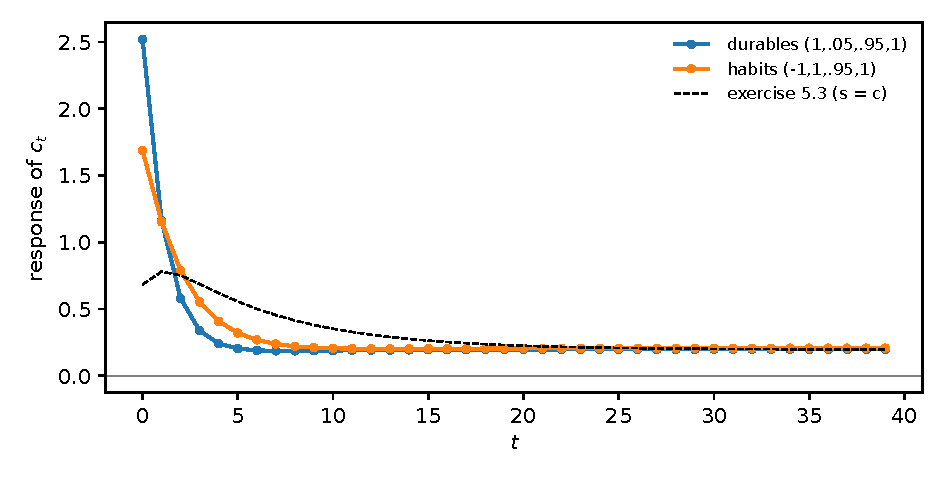
\includegraphics[width=0.8\linewidth]{fig/ls05_durables_habits.pdf}\\[3pt]
\captionof{figure}{Exercise 5.4. Response of $c_t$ to a unit shock to $y_0$, holding the other
states at zero.}
\label{fig:dur}
\end{center}
\end{tcolorbox}

%----------------------------------------------------------------------
\subsection{Discounted Sums and Values}
%----------------------------------------------------------------------

%------- 5.5 -------
\begin{tcolorbox}[oddbox,title={Exercise 5.5 \quad Expected discounted sum of an ARMA(2,1)}]
\begin{tcolorbox}[questionbox]
pp.~146--147. $y_{t+1}=\rho_1y_t+\rho_2y_{t-1}+w_{t+1}+\gamma w_t$, $w$ a unit-variance Gaussian
martingale difference. Compute $E\sum_{j\ge0}\beta^j[y_{t+j}\mid y^t,w^t]$: (a) write a program;
(b) evaluate at $(\beta,\rho_1,\rho_2,\gamma)=(.95,1.2,-.4,.5)$.
\end{tcolorbox}

\textbf{Solution:}

\textbf{(a)} State $x_t=[y_t,\ y_{t-1},\ w_t]'$ (the MA term needs $w_t$). Then
\[
x_{t+1}=\underbrace{\begin{bmatrix}\rho_1&\rho_2&\gamma\\1&0&0\\0&0&0\end{bmatrix}}_{A}x_t
+\underbrace{\begin{bmatrix}1\\0\\1\end{bmatrix}}_{C}w_{t+1},\qquad y_t=Gx_t,\ G=[1,0,0].
\]
Since $E_tw_{t+j}=0$ for $j\ge1$, $E_tx_{t+j}=A^jx_t$ and
\[
E_t\sum_{j\ge0}\beta^jy_{t+j}=G\sum_{j\ge0}(\beta A)^jx_t=G(I-\beta A)^{-1}x_t,
\]
valid when the eigenvalues of $A$ are below $1/\beta$ in modulus. The program computes the row
$g=G(I-\beta A)^{-1}$ by solving $g(I-\beta A)=G$.

\emph{Closed form.} Column by column, $g(I-\beta A)=G$ reads
$g_1(1-\beta\rho_1)-\beta g_2=1$, $-\beta\rho_2g_1+g_2=0$, $-\beta\gamma g_1+g_3=0$. So
$g_2=\beta\rho_2g_1$, $g_3=\beta\gamma g_1$, and
\[
g_1=\frac{1}{1-\beta\rho_1-\beta^2\rho_2}.
\]

\textbf{(b)} The eigenvalues of $A$ are $0$ and $0.6\pm0.2i$ (modulus $0.632<1/\beta$).
$1-\beta\rho_1-\beta^2\rho_2=1-1.14+0.361=0.221$, so
\[
\boxed{E_t\sum_j\beta^jy_{t+j}=4.52489\,y_t-1.71946\,y_{t-1}+2.14932\,w_t.}
\]
($g_2=-0.38\,g_1$, $g_3=0.475\,g_1$.) A 40\,000-path Monte Carlo from a fixed state matches
within its standard error.
\end{tcolorbox}

%------- 5.6 -------
\begin{tcolorbox}[evenbox,title={Exercise 5.6 \quad Finding the state is an art}]
\begin{tcolorbox}[questionbox]
p.~147. $d_{t+1}=\rho_0+\rho_1d_t+\rho_2d_{t-1}+\sigma_d\epsilon_{t+1}$,
$s_t=\beta^t(b_0-b_1d_t)$, $v_0=E_0\sum_ts_td_t$. (a) Describe a recursive algorithm for $v_0$.
(b) Give conditions on $\beta,\rho_1,\rho_2$ sufficient for $v_0<\infty$.
\end{tcolorbox}

\textbf{Solution:} (The statement gives initial conditions $d_0,d_1$ but conditions on
$d_0,d_{-1}$; we use $d_0,d_{-1}$, which is what the time-0 expectation requires.)

\textbf{(a) The state.} The summand $s_td_t=\beta^t(b_0d_t-b_1d_t^2)$ is a \emph{quadratic}
function of $d_t$ with a linear part, and $d$ is second order with a drift. The state that makes it
all quadratic in one vector is $x_t=[1,\ d_t,\ d_{t-1}]'$:
\[
x_{t+1}=\underbrace{\begin{bmatrix}1&0&0\\\rho_0&\rho_1&\rho_2\\0&1&0\end{bmatrix}}_{A}x_t+
\underbrace{\begin{bmatrix}0\\\sigma_d\\0\end{bmatrix}}_{C}\epsilon_{t+1},\qquad
b_0d_t-b_1d_t^2=x_t'Mx_t,\quad
M=\begin{bmatrix}0&b_0/2&0\\b_0/2&-b_1&0\\0&0&0\end{bmatrix}.
\]
Guess $v(x)=x'Px+\delta$ for $v(x_t)=E_t\sum_j\beta^jx_{t+j}'Mx_{t+j}$. The recursion
$v(x)=x'Mx+\beta E\,v(Ax+C\epsilon)$ and $E(Ax+C\epsilon)'P(Ax+C\epsilon)=x'A'PAx+\tr(PCC')$ give
\[
x'Px+\delta=x'(M+\beta A'PA)x+\beta\tr(PCC')+\beta\delta,
\]
so
\[
P=M+\beta A'PA,\qquad \delta=\frac{\beta}{1-\beta}\tr(PCC').
\]
\emph{Algorithm:} iterate $P_{j+1}=M+\beta A'P_jA$ from $P_0=0$ ($P_j$ is the $j$-period sum),
or solve the discrete Lyapunov equation directly (doubling algorithm); then
$v_0=x_0'Px_0+\beta(1-\beta)^{-1}\tr(PCC')$. This is (5.3.4)--(5.3.5) with no control and a
reward instead of a loss.

\textbf{(b)} $P=\sum_t\beta^tA'^tMA^t$. The eigenvalues of $A$ are $1$ (the constant) and the roots
$\lambda_1,\lambda_2$ of $\lambda^2-\rho_1\lambda-\rho_2=0$. The terms of $A'^tMA^t$ behave like
products $\lambda_i^t\lambda_j^t$ of pairs of eigenvalues that $M$ loads on (times powers of $t$ when
roots repeat). The $b_1d^2$ term needs $\beta|\lambda_i\lambda_j|<1$; the $b_0d$ term needs
$\beta|\lambda_i|<1$. A sufficient condition covering both and $\delta$:
\[
\boxed{\max\{|\lambda_1|,|\lambda_2|\}<\beta^{-1/2}\quad(\text{roots of }\lambda^2-\rho_1\lambda-\rho_2=0).}
\]
With $b_1=0$ the weaker $\max|\lambda_i|<\beta^{-1}$ suffices. A unit root is allowed: $d_t$ then
grows at most polynomially and $\beta^t$ still wins.

\begin{tcolorbox}[databox]
$\beta=.95$, $\rho_0=1$, $\rho_1=1.2$, $\rho_2=-.3$, $\sigma_d=.5$, $b_0=1$, $b_1=.02$ (our choice),
$x_0=[1,9,8.5]'$: $v_0=156.720$ (531 iterations; equal to \texttt{scipy}'s Lyapunov solver; Monte Carlo
$156.737\pm0.035$). With roots $\{1,0.9\}$ ($\beta\max|\lambda|^2=0.95$) the iteration converges;
with roots $\{1.05,0.5\}$ ($\beta\max|\lambda|^2=1.047$) it diverges, as the condition predicts.
\end{tcolorbox}
\end{tcolorbox}

%----------------------------------------------------------------------
\subsection{Money Finance and Tax Smoothing}
%----------------------------------------------------------------------

%------- 5.7 -------
\begin{tcolorbox}[oddbox,title={Exercise 5.7 \quad Dynamic Laffer curves}]
\begin{tcolorbox}[questionbox]
pp.~147--148. $M_t/p_t=\gamma_1-\gamma_2p_{t+1}/p_t$ (1), $(M_t-M_{t-1})/p_t=g$ (2), $M_{-1}=100$;
equilibrium: positive $\{p_t,M_t\}$ satisfying (1)--(2). (a) Program for
$\gamma_1=100,\gamma_2=50,g=.05$. (b) Continuum of equilibria; lowest $p_0$. (c) All but the minimal-$p_0$
equilibrium share the same limiting inflation and money growth; compute it. (d) The unique
equilibrium with lower inflation. (e) Redo with $g=.075$; do larger deficits cause more inflation?
(f) Discuss via the Laffer curve.
\end{tcolorbox}

\textbf{Solution:}

\textbf{A difference equation in $p$.} From (1), $M_t=\gamma_1p_t-\gamma_2p_{t+1}$ for $t\ge0$.
Substituting into (2) for $t\ge1$, $M_t-M_{t-1}=gp_t$:
\[
\gamma_1p_t-\gamma_2p_{t+1}-\gamma_1p_{t-1}+\gamma_2p_t=gp_t
\;\Longrightarrow\;
\gamma_2p_{t+1}-(\gamma_1+\gamma_2-g)p_t+\gamma_1p_{t-1}=0,\quad t\ge1.
\]
At $t=0$, (1)--(2) with $M_{-1}$ give $\gamma_1p_0-\gamma_2p_1-M_{-1}=gp_0$, i.e.
$p_1=[(\gamma_1-g)p_0-M_{-1}]/\gamma_2$. So $p_0$ is the only free initial condition.

\textbf{(a) Program.} Given $p_0$: for $t=0,1,\dots$ set $M_t=M_{t-1}+gp_t$ (budget) and
$p_{t+1}=(\gamma_1p_t-M_t)/\gamma_2$ (money demand); an equilibrium iff all $p_t,M_t>0$
(\texttt{equilibrium\_path} in the notebook). Independent route: the closed form below.

\textbf{Closed form.} The characteristic polynomial is
$\gamma_2\lambda^2-(\gamma_1+\gamma_2-g)\lambda+\gamma_1=0$; with the numbers,
$50\lambda^2-149.95\lambda+100=0$,
\[
\lambda=\frac{149.95\mp\sqrt{149.95^2-20\,000}}{100}=\frac{149.95\mp49.8498}{100},
\]
so $\lambda_1=1.001002$ and $\lambda_2=1.997998$
($\lambda_1\lambda_2=\gamma_1/\gamma_2=2$, $\lambda_1+\lambda_2=2.9990$). Hence
$p_t=c_1\lambda_1^t+c_2\lambda_2^t$ with $c_1+c_2=p_0$, $c_1\lambda_1+c_2\lambda_2=p_1$, so
\[
c_2=\frac{p_1-\lambda_1p_0}{\lambda_2-\lambda_1}
=\frac{p_0\big[\tfrac{\gamma_1-g}{\gamma_2}-\lambda_1\big]-\tfrac{M_{-1}}{\gamma_2}}{\lambda_2-\lambda_1}
=\frac{p_0(\lambda_2-1)-M_{-1}/\gamma_2}{\lambda_2-\lambda_1},
\]
using $\lambda_1+\lambda_2=1+(\gamma_1-g)/\gamma_2$.

\textbf{(b) A continuum; the lowest $p_0$.} Positivity of $M$ is automatic once prices are positive
($M_t=M_{t-1}+gp_t$ is then increasing from $M_{-1}>0$), and positive $M,p$ in (1) imply
$p_{t+1}/p_t<\gamma_1/\gamma_2$. So equilibrium $\iff p_t>0$ for all $t$. Since $\lambda_2>\lambda_1$,
$c_2<0$ drives $p_t\to-\infty$: not an equilibrium. If $c_2\ge0$, $p_t/\lambda_1^t=c_1+c_2(\lambda_2/\lambda_1)^t$
is nondecreasing and positive at $t=0$, so $p_t>0$ for all $t$. Hence every
\[
p_0\ \ge\ \underline p_0=\frac{M_{-1}}{\gamma_2(\lambda_2-1)}=\frac{100}{50\times0.997998}=\boxed{2.004012}
\]
is an equilibrium --- a continuum --- and no lower $p_0$ is (Hint~1). Section 5.5's method gives the
same number: $\underline p_0$ is the $p_0$ that sets to zero the coordinate of $(p_1,p_0)$ on the
unstable eigenvector of the companion matrix (checked in the notebook).

\textbf{(c)} For $p_0>\underline p_0$, $c_2>0$ and $p_{t+1}/p_t\to\lambda_2$. Money:
$M_t=\gamma_1p_t-\gamma_2p_{t+1}=c_1\lambda_1^t(\gamma_1-\gamma_2\lambda_1)+c_2\lambda_2^t(\gamma_1-\gamma_2\lambda_2)$,
also dominated by $\lambda_2^t$, so $M_t/M_{t-1}\to\lambda_2$. Common limit:
$\boxed{\lambda_2=1.997998}$, i.e.\ about 99.8\% inflation per period, with real balances
$\gamma_1-\gamma_2\lambda_2=0.1001$.

\textbf{(d)} At $p_0=\underline p_0$, $c_2=0$ and $p_t=\underline p_0\lambda_1^t$: constant gross inflation
$\boxed{\lambda_1=1.001002}$ (0.1\%) from $t=0$, real balances $49.95$. It is the only equilibrium whose
inflation does not converge to $\lambda_2$, hence the unique lower-inflation one.

\textbf{(e)} With $g=.075$: $50\lambda^2-149.925\lambda+100=0$ gives $\lambda_1=1.001505$,
$\lambda_2=1.996995$ ($\underline p_0=2.006027$). The low-inflation equilibrium's inflation
\emph{rises} with the deficit ($1.001002\to1.001505$); the limiting inflation of the continuum
\emph{falls} ($1.997998\to1.996995$). ``Larger permanent deficits cause larger inflation'' holds only
on the low-inflation equilibrium.

\textbf{(f) Laffer curve.} In a stationary equilibrium $\pi_{t+1}=\pi$, real balances are
$m=\gamma_1-\gamma_2\pi$ and (2) reads $m(1-1/\pi)=g$: seigniorage
\[
\mathcal S(\pi)=(\gamma_1-\gamma_2\pi)(1-1/\pi)=g
\;\iff\;\gamma_2\pi^2-(\gamma_1+\gamma_2-g)\pi+\gamma_1=0,
\]
the same polynomial: $\lambda_1,\lambda_2$ are the two inflation rates that raise $g$ in a steady
state. $\mathcal S'(\pi)=-\gamma_2+\gamma_1/\pi^2=0$ at $\pi^*=\sqrt{\gamma_1/\gamma_2}=\sqrt2$, where
$\mathcal S=(100-70.71)(1-0.7071)=8.58$. $\lambda_1<\pi^*$ is on the ``good'' side, where
more revenue needs more inflation; $\lambda_2>\pi^*$ is on the wrong side, where raising more revenue
means \emph{less} inflation because real balances expand. The continuum of equilibria all converge to
the wrong side; only the minimal-$p_0$ equilibrium stays on the good side.

\begin{center}
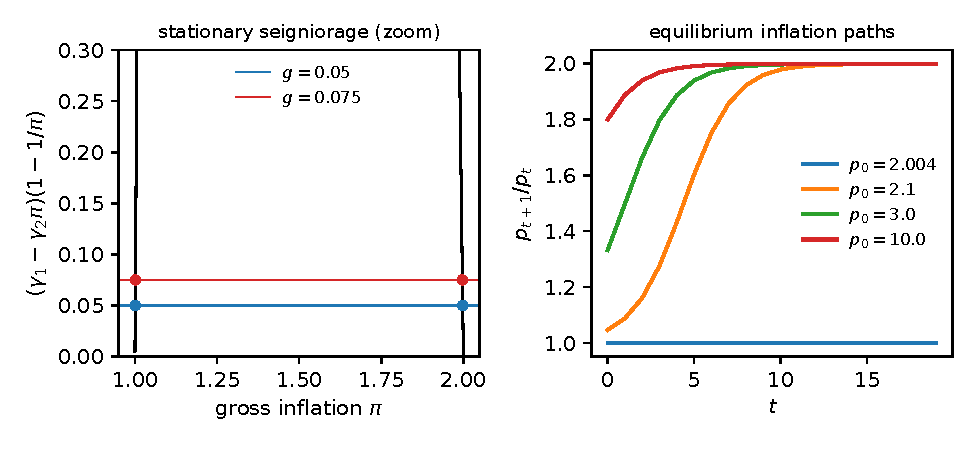
\includegraphics[width=0.95\linewidth]{fig/ls05_laffer.pdf}\\[3pt]
\captionof{figure}{Exercise 5.7. Left: stationary seigniorage (zoom near $\mathcal S=0$) and the two
roots for $g=.05$, $.075$. Right: gross inflation along equilibria with $p_0=\underline p_0$ and larger
$p_0$.}
\end{center}
\end{tcolorbox}

%------- 5.8 -------
\begin{tcolorbox}[evenbox,title={Exercise 5.8 \quad Tax smoothing and a VAR for $[g_t,T_t]$}]
\begin{tcolorbox}[questionbox]
pp.~149--150. $g_t=g_{Tt}+g_{Pt}$; $g_{P,t+1}=g_{Pt}+c_1\epsilon_{1,t+1}$,
$g_{T,t+1}=(1-\rho)\mu_T+\rho g_{Tt}+c_2\epsilon_{2,t+1}$. Minimise $E\sum_t\beta^tW(T_t)$,
$W(T)=w_1T+.5w_2T^2$, s.t.\ $g_t+qb_{t+1}=T_t+b_t$, $b_0=0$,
$\lim\beta^tW'(T_t)b_{t+1}=0$. (a) Bellman equation, state, control, strategy, forms of value
and rule. (b) Law of motion of $(g_{Tt},g_{Pt},T_t,b_{t+1})$. (c) Define the population VAR for
$[g_t,T_t]$. (d) How does it depend on $[\rho,\beta,\mu,q,w_1,w_2,c_1,c_2]$? (e) With a noisy
$\tilde b_t=b_t+c_3w_{3,t+1}$ added, how is the VAR related to the parameters; can it be used for
inference?
\end{tcolorbox}

\textbf{Solution:} Rearranging the budget, $b_t=g_t-T_t+qb_{t+1}$: $b_t$ is government
\emph{assets} (a claim that pays $b_t$ at $t$), and iterating forward under no-Ponzi,
$b_t=E_t\sum_jq^j(g_{t+j}-T_{t+j})$, i.e.\ $E_t\sum_jq^jT_{t+j}=E_t\sum_jq^jg_{t+j}-b_t$.

\textbf{(a)} State $x_t=[b_t,\ g_{Pt},\ g_{Tt},\ 1]'$; control $u_t=b_{t+1}$. Then
$T_t=Sx_t+qu_t$, $S=[-1,1,1,0]$. With $e_4=[0,0,0,1]$ (so $e_4x=1$),
\[
W(T_t)=w_1T_t+\tfrac12w_2T_t^2=x_t'Rx_t+u_t'Qu_t+2u_t'Hx_t,
\]
\[
R=\tfrac12w_2S'S+\tfrac12w_1(e_4'S+S'e_4),\qquad Q=\tfrac12w_2q^2,\qquad H=q\big(\tfrac12w_2S+\tfrac12w_1e_4\big),
\]
(expand $\tfrac12w_2(Sx+qu)^2+w_1(Sx+qu)\cdot e_4x$). Law of motion $x_{t+1}=Ax_t+Bu_t+C\epsilon_{t+1}$:
\[
A=\begin{bmatrix}0&0&0&0\\0&1&0&0\\0&0&\rho&(1-\rho)\mu_T\\0&0&0&1\end{bmatrix},\quad
B=\begin{bmatrix}1\\0\\0\\0\end{bmatrix},\quad
C=\begin{bmatrix}0&0\\c_1&0\\0&c_2\\0&0\end{bmatrix}.
\]
Bellman equation (loss written as a negative value):
\[
-x'Px-d=\max_u\big\{-x'Rx-u'Qu-2u'Hx+\beta E[-(Ax+Bu+C\epsilon)'P(Ax+Bu+C\epsilon)-d]\big\}.
\]
By Exercise~5.1 and certainty equivalence: value $v(x)=-x'Px-d$, $d=\beta(1-\beta)^{-1}\tr(PCC')$;
rule $b_{t+1}=-Fx_t$, $F=(Q+\beta B'PB)^{-1}(\beta B'PA+H)$; $T_t=(S-qF)x_t$. \emph{Strategy:}
Howard's algorithm from a stable rule, or the stabilising DARE solution (not the Riccati iteration
from $P_0=0$ --- see the trap box).

\emph{Closed form when $q=\beta$} (the natural case: the government discounts at the market rate).
The Euler equation for $b_{t+1}$ is $qW'(T_t)=\beta E_tW'(T_{t+1})$, i.e.\
$w_1+w_2T_t=w_1+w_2E_tT_{t+1}$: \textbf{taxes are a martingale}, $E_tT_{t+j}=T_t$. Then
$E_t\sum q^jT_{t+j}=T_t/(1-q)$ and, using
$E_tg_{P,t+j}=g_{Pt}$, $E_tg_{T,t+j}=\mu_T+\rho^j(g_{Tt}-\mu_T)$:
\[
\boxed{T_t=g_{Pt}+\mu_T+\kappa(g_{Tt}-\mu_T)-(1-q)b_t,\qquad \kappa=\frac{1-q}{1-q\rho}.}
\]
$w_1$ and $w_2$ do not appear. (If $q\ne\beta$, $W'(T_t)=(\beta/q)E_tW'(T_{t+1})$ tilts the tax
path and the rule depends on $w_1/w_2$ --- never on the scale of $W$.)

\textbf{(b)} Under the rule, $x_{t+1}=(A-BF)x_t+C\epsilon_{t+1}$, $T_t=(S-qF)x_t$, $b_{t+1}=-Fx_t$,
$g_t=[0,1,1,0]x_t$. At $q=\beta$ explicitly: substituting $T_t$ into the budget,
$qb_{t+1}=T_t+b_t-g_t=qb_t+(\kappa-1)(g_{Tt}-\mu_T)$ and $\kappa-1=-q(1-\rho)/(1-q\rho)$, so
$b_{t+1}=b_t-\frac{1-\rho}{1-q\rho}(g_{Tt}-\mu_T)$,
and
\[
T_{t+1}-T_t=c_1\epsilon_{1,t+1}+\kappa c_2\epsilon_{2,t+1}
\]
(the drift terms cancel: $\kappa(\rho-1)+(1-q)(1-\rho)/(1-q\rho)=0$). Permanent spending shocks pass
one-for-one into taxes; transitory ones only by the annuity factor $\kappa$; debt absorbs the rest.

\textbf{(c)} Let $z_t=[g_t,T_t]'$. The population VAR is the projection
$z_{t+1}=\nu+\sum_{j\ge0}\mathcal A_jz_{t-j}+a_{t+1}$ with $a_{t+1}=z_{t+1}-\hat E[z_{t+1}\mid z^t]$
orthogonal to all past $z$. It is obtained from the state space
$x_{t+1}=A_ox_t+C\epsilon_{t+1}$, $z_t=Gx_t$ ($A_o=A-BF$, $G$ stacks $[0,1,1,0]$ and $S-qF$) with
the steady-state Kalman filter (5.6.2)--(5.6.4): $\hat x_{t+1}=A_o\hat x_t+Ka_t$, $z_t=G\hat x_t+a_t$.
Inverting, $\hat x_{t+1}=(A_o-KG)\hat x_t+Kz_t$, so
\[
\mathcal A_j=G(A_o-KG)^jK,\qquad Ea_ta_t'=G\Sigma G'.
\]

\textbf{(d)} The VAR is a function of $(A_o,C,G)$ only, i.e.\ of $(\rho,\mu_T,q,c_1,c_2)$ and of the
rule. At $q=\beta$ the rule does not involve $w_1,w_2$ and $\beta$ enters only as $q$: the VAR is
\emph{identical} for all $(w_1,w_2)$, which are therefore not identified; this is the cross-equation
restriction the theory imposes. A subtler point: the VAR innovations are \emph{not} the
$\epsilon$'s. $g-T$ loads on $\epsilon_2$ through a polynomial with root $L=q$ inside the unit
circle, so the shocks are not recoverable from current and past $(g,T)$. In the filter this shows up
as $A_o-KG$ having the root $q$ (the iteration started from $\Sigma=CC'$ lands instead on a
non-stabilising fixed point with root $1/q$), and $\mathrm{Var}(a_g)>\mathrm{Var}(c_1\epsilon_1+c_2\epsilon_2)$.

\textbf{(e)} Now $z_t=[g_t,T_t,\tilde b_t]'$ with $\tilde b_t=[1,0,0,0]x_t+c_3w_{3,t+1}$: the same
state space with measurement noise $v_t$, $Ev_tv_t'=\mathrm{diag}(0,0,c_3^2)$. The VAR is again
$\mathcal A_j=G(A_o-KG)^jK$, with $K,\Sigma$ from (5.6.3) with $R=\mathrm{diag}(0,0,c_3^2)$, and
depends on $(\rho,\mu_T,q,c_1,c_2,c_3)$ (plus $w_1/w_2$ and $\beta$ only if $q\ne\beta$). Inference:
yes --- not by reading parameters off OLS coefficients, but by maximum likelihood on the state space,
the Gaussian likelihood being $\prod_t N(a_t;0,G\Sigma_tG'+R)$ from the Kalman filter (as in
5.9). The debt series pins down the hidden state and sharpens the estimates of $(\rho,\mu_T,c_1,c_2)$;
$w_1,w_2$ remain unidentified at $q=\beta$.

\begin{tcolorbox}[databox]
$\beta=q=.95$, $\rho=.8$, $\mu_T=.1$, $c_1=.01$, $c_2=.03$, $w_1=1$, $w_2=2$ (our choice).
LQ (DARE, and Howard from $b_{t+1}=b_t$ in 2 steps): $T_t=-0.05b_t+g_{Pt}+0.20833g_{Tt}+0.07917$ =
closed form ($\kappa=0.20833$); unchanged for $(w_1,w_2)=(0,1),(3,.5)$; $E_tT_{t+1}=T_t$ exactly.
VAR: $\mathcal A_0=\begin{bmatrix}0.850&0.040\\0&1\end{bmatrix}$, eigenvalues of $A_o-KG$
$\{0.95,1,0,0\}$, $\mathrm{Var}(a_g)=1.04\times10^{-3}$ vs $c_1^2+c_2^2=1.00\times10^{-3}$. A 40-lag
OLS VAR on 200\,000 simulated periods gives lag-1 matrix $\begin{bmatrix}0.850&0.041\\0.001&0.996\end{bmatrix}$
and the same innovation covariance. Adding $\tilde b$ with $c_3=.1$ cuts $\tr\Sigma$ from $0.307$
to $0.002$.
\end{tcolorbox}

\begin{tcolorbox}[trapbox]
\begin{itemize}[itemsep=2pt]
\item \textbf{The Riccati iteration from $P_0=0$ finds a Ponzi scheme.} $W$ has its minimum at
$T=-w_1/w_2$; setting $T_t\equiv-w_1/w_2$ and letting assets fall at rate $1/q$ gives $W'\equiv0$, so the
stated terminal condition $\beta^tW'(T_t)b_{t+1}\to0$ holds trivially. The iteration converges to
exactly this rule (closed-loop root $1/q>1/\sqrt\beta$). The intended condition is no-Ponzi,
$q^tb_{t+1}\to0$, which in the regulator means selecting the stabilising solution.
\item \textbf{VAR shocks $\ne$ structural shocks} (non-invertibility, root $q$).
\end{itemize}
\end{tcolorbox}
\end{tcolorbox}

%----------------------------------------------------------------------
\subsection{Planning, Estimation and Policy Improvement}
%----------------------------------------------------------------------

%------- 5.9 -------
\begin{tcolorbox}[oddbox,title={Exercise 5.9 \quad A permanent-income planner and its likelihood}]
\begin{tcolorbox}[questionbox]
pp.~150--152. Maximise $-.5E_0\sum_t\beta^t[(c_t-b_t)^2+ei_t^2]$ s.t.\ $c_t+i_t=\gamma k_t+d_t$,
$k_{t+1}=(1-\delta)k_t+i_t$, $b_{t+1}=\mu_b(1-\rho_b)+\rho_bb_t+\sigma_b\epsilon_{b,t+1}$,
$d_{t+1}=\mu_d(1-\rho_d)+\rho_dd_t+\sigma_d\epsilon_{d,t+1}$, and ``$\beta\gamma(1-\delta)=1$''.
Part I: (a) dynamic program; (b) effects of $\sigma_b,\sigma_d$ on the rules; (c) algorithm.
Part II: an econometrician sees $\{c_t,i_t\}_{t=0}^T$, not $k,b,d$, with
$[k_0,b_0,d_0]'\sim N(\mu_0,\Sigma_0)$, knows $\beta$. (a) Maximum likelihood, recursively;
(b) Bayesian posterior algorithm.
\end{tcolorbox}

\textbf{Solution:} \emph{Reading.} Substituting $i_t$, $k_{t+1}=(1-\delta+\gamma)k_t+d_t-c_t$: the
gross return on capital is $1-\delta+\gamma$, so the Hall--Friedman condition ``$\beta R=1$'' is
$\beta(1-\delta+\gamma)=1$. We read the printed $\beta\gamma(1-\delta)=1$ as this (with the literal
version the gross return would be about 2 for $\delta=.1$); nothing in the method depends on it.

\textbf{Part I (a).} State $x_t=[k_t,\ b_t,\ d_t,\ 1]'$, control $u_t=i_t$. $c_t-b_t=Sx_t-u_t$ with
$S=[\gamma,-1,1,0]$, so the return is $-\tfrac12[(Sx-u)^2+eu^2]=-(x'Rx+u'Qu+2u'Hx)$ with
\[
R=\tfrac12S'S,\qquad Q=\tfrac12(1+e),\qquad H=-\tfrac12S,
\]
\[
A=\begin{bmatrix}1-\delta&0&0&0\\0&\rho_b&0&\mu_b(1-\rho_b)\\0&0&\rho_d&\mu_d(1-\rho_d)\\0&0&0&1\end{bmatrix},\quad
B=\begin{bmatrix}1\\0\\0\\0\end{bmatrix},\quad
C=\begin{bmatrix}0&0\\\sigma_b&0\\0&\sigma_d\\0&0\end{bmatrix}.
\]
Bellman equation:
$v(x)=\max_u\{-x'Rx-u'Qu-2u'Hx+\beta E\,v(Ax+Bu+C\epsilon)\}$, solved by $v=-x'Px-\varrho$ with $P$ from
(1) of Exercise~5.1, $\varrho=\beta(1-\beta)^{-1}\tr(PCC')$, and $i_t=-Fx_t$,
$c_t=(S+F)x_t+b_t$.

\textbf{(b)} By certainty equivalence (section 5.3, which carries over with the cross term since
$E\epsilon=0$): $P$ and $F$ do not depend on $C$. An increase in $\sigma_b$ or $\sigma_d$ leaves the
decision rules for $c_t$ and $k_{t+1}$ \emph{unchanged}; it only raises
$\varrho=\beta(1-\beta)^{-1}(P_{22}\sigma_b^2+P_{33}\sigma_d^2)$, lowering the value. No precautionary
saving.

\textbf{(c)} Iterate (1) of 5.1 from $P_0=0$, or Howard's algorithm from a stable rule, or the Schur
method $P=V_{21}V_{11}^{-1}$ of section 5.5; then $F$ and $\varrho$ as above.

\textbf{Part II (a) Maximum likelihood.} For given $\theta$: solve Part I for $F(\theta)$; form the
closed loop $x_{t+1}=A_o(\theta)x_t+C(\theta)\epsilon_{t+1}$, $A_o=A-BF$, and the observation
$z_t=[c_t,i_t]'=G(\theta)x_t$ with rows $S+F+[0,1,0,0]$ and $-F$. No measurement error; two shocks,
two observables. Kalman filter (5.6.2)--(5.6.3) with $R=0$, started at $\hat x_0=[\mu_0',1]'$,
$\Sigma_0=\mathrm{diag}(\Sigma_0,0)$:
\begin{gather*}
a_t=z_t-G\hat x_t,\qquad \Omega_t=G\Sigma_tG',\qquad K_t=A_o\Sigma_tG'\Omega_t^{-1},\\
\hat x_{t+1}=A_o\hat x_t+K_ta_t,\qquad \Sigma_{t+1}=A_o\Sigma_tA_o'+CC'-K_t\Omega_tK_t'.
\end{gather*}
Since $z_t\mid z^{t-1}\sim N(G\hat x_t,\Omega_t)$, the likelihood factors recursively:
\[
\log L(\theta)=-\sum_{t=0}^T\Big[\log2\pi+\tfrac12\log\det\Omega_t+\tfrac12a_t'\Omega_t^{-1}a_t\Big].
\]
Maximise over $\theta$ (minus $\beta$, and with $\gamma=1/\beta-1+\delta$ imposed) by a numerical
optimiser; each evaluation solves a Riccati equation and runs the filter. Standard errors from the
inverse Hessian.

\textbf{(b) Bayesian.} Posterior $p(\theta\mid z^T)\propto L(\theta)p(\theta)$. Random-walk
Metropolis--Hastings: start at $\theta^{(0)}$ (e.g.\ the MLE); at step $s$ draw
$\theta^*=\theta^{(s)}+\eta$, $\eta\sim N(0,c\hat V)$ ($\hat V$ the inverse Hessian); compute
$\log L(\theta^*)$ with the filter; accept with probability
$\min\{1,\,L(\theta^*)p(\theta^*)/[L(\theta^{(s)})p(\theta^{(s)})]\}$ (reject draws with
$\rho_b,\rho_d\notin(0,1)$, $e\le0$, etc.); otherwise keep $\theta^{(s)}$. Discard a burn-in; the
remaining draws approximate the posterior. Tune $c$ for a 20--40\% acceptance rate.

\begin{tcolorbox}[databox]
$\beta=.95$, $\delta=.1$, $\gamma=1/\beta-1+\delta$, $e=1$, $\mu_b=30$, $\mu_d=5$, $\rho_b=.9$,
$\rho_d=.8$, $\sigma_b=\sigma_d=1$ (our choice): $i_t=0.0368k_t-0.2410b_t+0.3331d_t+5.5653$;
eigenvalues of $A-BF$: $0.937,0.9,0.8,1$. Raising $\sigma_b$ or $\sigma_d$ to 3 leaves $F,P$
unchanged; $\varrho$ goes from 54.85 to 344.65 and 203.89. Kalman log-likelihood of 13 simulated
observations $=-22.131962$, equal to the direct Gaussian density of the stacked vector. On 601
observations the profile likelihood in $\rho_b$ peaks at $0.905$ (true $0.9$)
(Figure~\ref{fig:lik}).
\end{tcolorbox}
\begin{center}
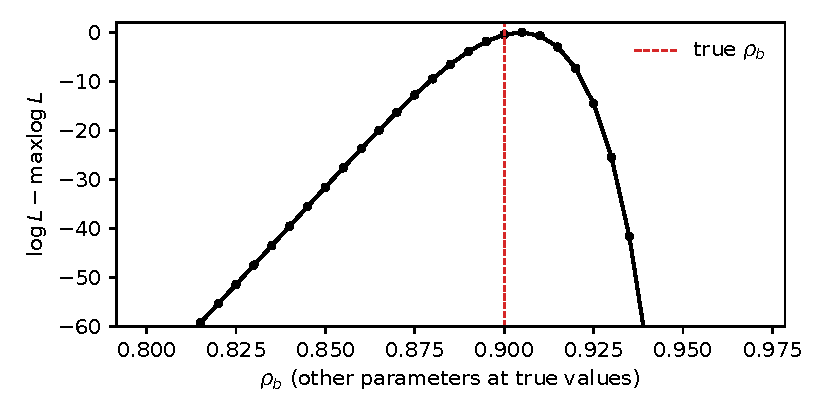
\includegraphics[width=0.7\linewidth]{fig/ls05_likelihood.pdf}\\[3pt]
\captionof{figure}{Exercise 5.9. Profile log-likelihood in $\rho_b$ from the Kalman filter.}
\label{fig:lik}
\end{center}
\end{tcolorbox}

%------- 5.10 -------
\begin{tcolorbox}[evenbox,title={Exercise 5.10 \quad Valuing a rule of thumb, then improving it}]
\begin{tcolorbox}[questionbox]
p.~152. Criterion $-.5E_0\sum_t\beta^t(c_t-b)^2$; $k_{t+1}=R(k_t+y_t-c_t)$,
$y_{t+1}=\mu_y(1-\rho_1-\rho_2)+\rho_1y_t+\rho_2y_{t-1}+\sigma_y\epsilon_{t+1}$, prescribed rule
$c_t=\alpha y_t+(R-1)k_t$. (a) Compute the value under the rule (Bellman equation, as far as
possible). (b) Use Howard's algorithm to get a better rule.
\end{tcolorbox}

\textbf{Solution:}

\textbf{(a)} State $x_t=[k_t,\ y_t,\ y_{t-1},\ 1]'$. Under the rule,
$k_t+y_t-c_t=(2-R)k_t+(1-\alpha)y_t$, so
\[
x_{t+1}=A_0x_t+C\epsilon_{t+1},\quad
A_0=\begin{bmatrix}R(2-R)&R(1-\alpha)&0&0\\0&\rho_1&\rho_2&\mu_y(1-\rho_1-\rho_2)\\0&1&0&0\\0&0&0&1\end{bmatrix},\quad
C=\begin{bmatrix}0\\\sigma_y\\0\\0\end{bmatrix},
\]
and $c_t-b=S_0x_t$, $S_0=[R-1,\ \alpha,\ 0,\ -b]$. The value satisfies the (control-free) Bellman
equation $v(x)=-\tfrac12(S_0x)^2+\beta E\,v(A_0x+C\epsilon)$. Guess $v=-x'P_0x-d_0$:
\[
x'P_0x+d_0=\tfrac12x'S_0'S_0x+\beta x'A_0'P_0A_0x+\beta\tr(P_0CC')+\beta d_0,
\]
so
\[
P_0=\tfrac12S_0'S_0+\beta A_0'P_0A_0,\qquad d_0=\frac{\beta\tr(P_0CC')}{1-\beta}.
\]
$P_0=\sum_t\beta^tA_0'^t(\tfrac12S_0'S_0)A_0^t$ exists iff the eigenvalues of $A_0$ --- $R(2-R)$,
the roots of the $y$ process, and 1 --- are below $1/\sqrt\beta$; with $R=1/\beta$,
$R(2-R)=0.997<1$.

\textbf{(b)} Now let $u_t=c_t$ be free: $x_{t+1}=Ax_t+Bu_t+C\epsilon_{t+1}$ with $A$'s first row
$[R,R,0,0]$ and $B=[-R,0,0,0]'$; the return $-\tfrac12(u-b\cdot e_4x)^2$ has $R_x=\tfrac12b^2e_4'e_4$,
$Q=\tfrac12$, $H=-\tfrac12b\,e_4$. Howard: start from $F_0=-[R-1,\alpha,0,0]$ (the prescribed rule,
$c=-F_0x$), with value $P_0$ from (a). Improve:
\[
F_{j+1}=(Q+\beta B'P_jB)^{-1}(\beta B'P_jA+H),
\]
evaluate $P_{j+1}=R_x+F'QF-H'F-F'H+\beta(A-BF)'P_{j+1}(A-BF)$ at $F=F_{j+1}$ (a Lyapunov equation),
repeat until $F$ stops changing. Each step weakly raises the value (Exercise 5.2).

\emph{Where it goes.} The limit is the permanent-income rule. With $\beta R=1$ the Euler equation
is $E_tc_{t+1}=c_t$; the budget iterated forward (no-Ponzi) is
$k_t=\sum_{j\ge0}R^{-j}E_t(c_{t+j}-y_{t+j})$, so
\[
c_t=(1-\beta)\Big[k_t+E_t\sum_j\beta^jy_{t+j}\Big],\qquad E_t\sum_j\beta^jy_{t+j}=e_1(I-\beta A_y)^{-1}[y_t,y_{t-1},1]'.
\]

\begin{tcolorbox}[databox]
$\beta=.95$, $R=1/\beta$, $b=3$, $\alpha=.5$, $\mu_y=1$, $\rho_1=1.2$, $\rho_2=-.3$, $\sigma_y=.1$ (our
choice). Value of the rule at $x_0=[2,1.1,1,1]'$: $-37.2088$ (Lyapunov; Monte Carlo
$-37.229\pm0.029$). Howard: first improvement $c=0.0501k+0.3872y_t-0.1104y_{t-1}+0.6994$; converges
in 5 improvements to $c=0.05k+0.38241y_t-0.10899y_{t-1}+0.72658$, exactly the PIH formula;
closed-loop roots $1,1,0.845,0.355$.
\end{tcolorbox}
\begin{tcolorbox}[trapbox]
The Riccati iteration from $P_0=0$ on this problem returns $P=0$, $c_t\equiv b$: consume the bliss
level forever and borrow without limit ($k$ explodes at rate $R$). The problem as posed has no
borrowing limit, and this Ponzi plan attains the upper bound 0. Howard's algorithm started from a
stable rule never leaves the class of stable rules, which is how it imposes the no-Ponzi condition
implicitly.
\end{tcolorbox}
\end{tcolorbox}

%----------------------------------------------------------------------
\subsection{Firms with Adjustment Costs}
%----------------------------------------------------------------------

%------- 5.11 -------
\begin{tcolorbox}[oddbox,title={Exercise 5.11 \quad Firm-level adjustment costs}]
\begin{tcolorbox}[questionbox]
pp.~152--153. A price-taking firm maximises $\sum_t\beta^t[p_ty_t-.5d(y_{t+1}-y_t)^2]$,
$p_t=A_0-A_1Y_t$, believes $Y_{t+1}=H_0+H_1Y_t$. (a) Bellman equation. (b) Value and rule for
$\beta=.95,d=2,A_0=100,A_1=1,H_0=200,H_1=.8$.
\end{tcolorbox}

\textbf{Solution:}

\textbf{(a)}
\[
v(y,Y)=\max_{y'}\big\{(A_0-A_1Y)y-\tfrac d2(y'-y)^2+\beta v(y',Y')\big\},\qquad Y'=H_0+H_1Y.
\]
Regulator form: $x_t=[y_t,\ Y_t,\ 1]'$, $u_t=y_{t+1}-y_t$. Return
$p_ty_t-\tfrac d2u_t^2=-(x_t'Rx_t+u_t'Qu_t)$ with
\[
R=\begin{bmatrix}0&A_1/2&-A_0/2\\A_1/2&0&0\\-A_0/2&0&0\end{bmatrix},\quad Q=\frac d2,\quad
A=\begin{bmatrix}1&0&0\\0&H_1&H_0\\0&0&1\end{bmatrix},\quad B=\begin{bmatrix}1\\0\\0\end{bmatrix}.
\]
$R$ is indefinite (revenue is linear in $y$), but the problem is well posed: output only enters
linearly, adjustment is penalised quadratically.

\textbf{Euler equation route.} Raising $y_{t+1}$ by one: $-d(y_{t+1}-y_t)+\beta[p_{t+1}+d(y_{t+2}-y_{t+1})]=0$,
i.e.\ $\Delta_t=\tfrac\beta dp_{t+1}+\beta\Delta_{t+1}$ with $\Delta_t\equiv y_{t+1}-y_t$. Solving
forward, $\Delta_t=\frac1d\sum_{j\ge0}\beta^{j+1}p_{t+1+j}$. With $\bar Y=H_0/(1-H_1)$ and
$Y_{t+s}=\bar Y+H_1^s(Y_t-\bar Y)$,
\[
\boxed{y_{t+1}-y_t=\frac1d\Big[\frac{\beta(A_0-A_1\bar Y)}{1-\beta}-\frac{\beta H_1A_1}{1-\beta H_1}(Y_t-\bar Y)\Big].}
\]
The rule does not depend on $y_t$; hence the value is linear in $y$:
$\partial v/\partial y_t=\sum_s\beta^sp_{t+s}=\frac{A_0}{1-\beta}-A_1\Big[\frac{\bar Y}{1-\beta}+\frac{Y_t-\bar Y}{1-\beta H_1}\Big]$,
so in $v=-x'Px$: $P_{yy}=0$, $-2P_{yY}=-A_1/(1-\beta H_1)$,
$-2P_{y1}=A_0/(1-\beta)-A_1\bar Y[1/(1-\beta)-1/(1-\beta H_1)]$.

\textbf{(b)} $\bar Y=1000$, $A_0-A_1\bar Y=-900$, $\beta/(1-\beta)=19$, $\beta H_1/(1-\beta H_1)=.76/.24=3.1667$:
\[
y_{t+1}-y_t=\tfrac12[-17\,100-3.1667(Y_t-1000)]=-6966.67-1.58333\,Y_t .
\]
The Riccati iteration (562 steps) gives the same rule and
\[
P=\begin{bmatrix}0&2.08333&6916.67\\2.08333&-6.39527&-50\,011.0\\6916.67&-50\,011.0&-1.35563\times10^{9}\end{bmatrix},
\qquad v(y,Y)=-x'Px,
\]
matching the closed-form entries ($-2P_{yY}=-4.1667=-1/0.24$; $-2P_{y1}=2000-1000(20-4.1667)=-13\,833.3$)
and a direct simulation of the discounted profits to $10^{-9}$.

\emph{Remark.} These parameters send the market price to $A_0-A_1\bar Y=-900<0$; with no
nonnegativity constraint the firm responds by driving $y$ to large negative values, which is why the
constant in the rule and the value are huge. The formulas are right; the economics of the chosen
numbers is odd.
\end{tcolorbox}

%------- 5.12 -------
\begin{tcolorbox}[evenbox,title={Exercise 5.12 \quad Adjustment costs with a demand shock}]
\begin{tcolorbox}[questionbox]
pp.~153--154. As 5.11 with $p_t=A_0-A_1Y_t+u_t$, $u_{t+1}=\rho u_t+\sigma_u\epsilon_{t+1}$,
$Y_{t+1}=H_0+H_1Y_t+H_2u_t$. (a) Bellman equation. (b) Value and rule for 5.11's numbers and
$H_2=2,\rho=.9,\sigma_u=.05$.
\end{tcolorbox}

\textbf{Solution:}

\textbf{(a)} The firm sees $p_t,Y_t$, hence $u_t=p_t-A_0+A_1Y_t$. State $x_t=[y_t,Y_t,u_t,1]'$:
\[
v(y,Y,u)=\max_{y'}\big\{(A_0-A_1Y+u)y-\tfrac d2(y'-y)^2+\beta E\,v(y',H_0+H_1Y+H_2u,\ \rho u+\sigma_u\epsilon')\big\}.
\]
Regulator: as 5.11 with the extra entry $R_{yu}=R_{uy}=-\tfrac12$ (for the $+uy$ revenue),
$A=\begin{bmatrix}1&0&0&0\\0&H_1&H_2&H_0\\0&0&\rho&0\\0&0&0&1\end{bmatrix}$, $B=e_1$,
$C=[0,0,\sigma_u,0]'$. Value $v=-x'Px-\varrho$, $\varrho=\beta(1-\beta)^{-1}\sigma_u^2P_{uu}$; rule $u=-Fx$.

\textbf{Closed form by certainty equivalence.} The Euler equation now holds in expectation:
$\Delta_t=\frac1d\sum_{j\ge0}\beta^{j+1}E_tp_{t+1+j}$. With $z_t=[Y_t,u_t,1]'$,
$z_{t+1}=A_zz_t+\text{noise}$, $A_z=\begin{bmatrix}H_1&H_2&H_0\\0&\rho&0\\0&0&1\end{bmatrix}$ and
$p_t=g'z_t$, $g=[-A_1,1,A_0]'$:
\[
\boxed{y_{t+1}-y_t=\frac1d\,g'\,\beta A_z(I-\beta A_z)^{-1}z_t,}\qquad
\frac{\partial v}{\partial y}=g'(I-\beta A_z)^{-1}z_t .
\]

\textbf{(b)} Numerically (both routes agree to $10^{-7}$):
\[
y_{t+1}-y_t=-6966.67-1.58333\,Y_t-24.3506\,u_t,
\]
the $Y$ and constant coefficients are those of 5.11 (a shock-free $u=0$ reproduces 5.11), and
\[
P=\begin{bmatrix}0&2.0833&23.851&6916.7\\2.0833&-6.3953&-152.77&-50\,011\\
23.851&-152.77&-4944.6&-2.0222\times10^6\\6916.7&-50\,011&-2.0222\times10^6&-1.3556\times10^9\end{bmatrix},
\]
and $\varrho=19\times0.0025\times(-4944.6)=-234.87$.
$\varrho<0$: the value is \emph{raised} by demand volatility, because $v$ is convex in $u$ (the firm
adjusts output to shocks). $\sigma_u$ changes $\varrho$ only, never the rule. Monte Carlo of the
discounted profits at $x_0=[10,50,0.2,1]'$ matches $-x_0'Px_0-\varrho$ within two standard errors.
(The $u$-coefficient: $H_2=2$ makes a positive demand shock raise future market output, lowering
future prices, which is why $u_t$ \emph{lowers} planned output growth.)
\end{tcolorbox}

%----------------------------------------------------------------------
\subsection{Permanent Income}
%----------------------------------------------------------------------

%------- 5.13 -------
\begin{tcolorbox}[oddbox,title={Exercise 5.13 \quad Permanent income model}]
\begin{tcolorbox}[questionbox]
p.~154. Maximise $E_0\sum_t\beta^t\{-.5(c_t-b)^2-.5\epsilon a_t^2\}$ s.t.\ $a_{t+1}+c_t=Ra_t+y_t$,
$y_{t+1}=(1-\rho_1-\rho_2)+\rho_1y_t+\rho_2y_{t-1}+\sigma_y\epsilon_{t+1}$, $R=\beta^{-1}$.
(a) Bellman equation. (b) Value and rule for $b=1000,\beta=.95,\rho_1=1.2,\rho_2=-.4,\sigma_y=.05,
\epsilon=10^{-6}$. (c) Eigenvalues of $A-BF$. (d) Same with $\epsilon=0$; compare.
\end{tcolorbox}

\textbf{Solution:}

\textbf{(a)} State $x_t=[a_t,\ y_t,\ y_{t-1},\ 1]'$, control $u_t=c_t$:
\[
v(a,y,y_{-1})=\max_c\big\{-\tfrac12(c-b)^2-\tfrac12\epsilon a^2+\beta E\,v(Ra+y-c,\ y',\ y)\big\}.
\]
Regulator: $R_x=\tfrac12\epsilon\,e_1'e_1+\tfrac12b^2e_4'e_4$, $Q=\tfrac12$, $H=-\tfrac12b\,e_4$ (from
$\tfrac12(c-b)^2=\tfrac12c^2-bc\cdot1+\tfrac12b^2$),
\[
A=\begin{bmatrix}R&1&0&0\\0&\rho_1&\rho_2&1-\rho_1-\rho_2\\0&1&0&0\\0&0&0&1\end{bmatrix},\quad
B=\begin{bmatrix}-1\\0\\0\\0\end{bmatrix},\quad C=\begin{bmatrix}0\\\sigma_y\\0\\0\end{bmatrix}.
\]
Value $v=-x'Px-d$, $d=\beta(1-\beta)^{-1}\sigma_y^2P_{22}$; rule $c=-Fx$.

\textbf{(b)} Riccati iteration from $P_0=0$ (772 steps; DARE agrees):
\[
c_t=0.05265\,a_t+0.22631\,y_t-0.08600\,y_{t-1}+0.85968,
\]
\[
P=\begin{bmatrix}0.02771&0.11911&-0.04526&-525.86\\0.11911&0.51202&-0.19456&-2260.50\\
-0.04526&-0.19456&0.07393&858.99\\-525.86&-2260.50&858.99&9\,982\,813\end{bmatrix},\qquad d=0.0243 .
\]

\textbf{(c)} Eigenvalues of $A-BF$: $0.99998$, $0.6\pm0.2i$ (modulus $0.632$), $1$. The last is the
constant; $0.6\pm0.2i$ are the income roots (unaffected by the choice); $0.99998$ is assets ---
nearly a unit root, the Hall random-walk property ($c$ inherits it).

\textbf{(d) $\epsilon=0$.} Now $R_x-H'Q^{-1}H=\tfrac12b^2e_4'e_4-\tfrac12b^2e_4'e_4=0$, so from
$P_0=0$ the iteration gives $F=Q^{-1}H$, i.e.\ $c_t=b$, and $P_1=0$ again: \textbf{$P=0$, $c_t\equiv
1000$, value 0}. Assets evolve as $a_{t+1}=Ra_t+y_t-1000$: a Ponzi scheme, closed-loop root
$R=1.0526>1/\sqrt\beta$. It is the sup of the problem as literally posed, because nothing rules out
unbounded debt. The algebraic Riccati equation has a second solution, the \emph{stabilising} one,
which is Hall's rule:
\[
c_t=(1-\beta)\Big[Ra_t+E_t\sum_j\beta^jy_{t+j}\Big]=0.05263\,a_t+0.22624\,y_t-0.08597\,y_{t-1}+0.85973,
\]
(derivation: $E_tc_{t+1}=c_t$ from $\beta R=1$; $Ra_t=\sum_jR^{-j}E_t(c_{t+j}-y_{t+j})$ under
no-Ponzi; $E_t\sum\beta^jy_{t+j}$ as in Exercise 5.5 with $g_1=1/0.221=4.5249$, so
$0.05\times4.5249=0.22624$, $0.05\times(-0.38)(4.5249)=-0.08597$). Its closed-loop roots are
$1,1,0.6\pm0.2i$: an exact unit root in assets. Comparison with (b): the $\epsilon=10^{-6}$ rule
differs from Hall's by at most $7\times10^{-5}$. \emph{The tiny penalty is a device} that makes
Ponzi schemes infinitely costly (the penalty grows like $\beta^tR^{2t}=\beta^{-t}$), so that the
limit of the Riccati iteration is the stabilising solution; as $\epsilon\downarrow0$ it selects
Hall's rule, not the $\epsilon=0$ iteration limit.

\begin{center}
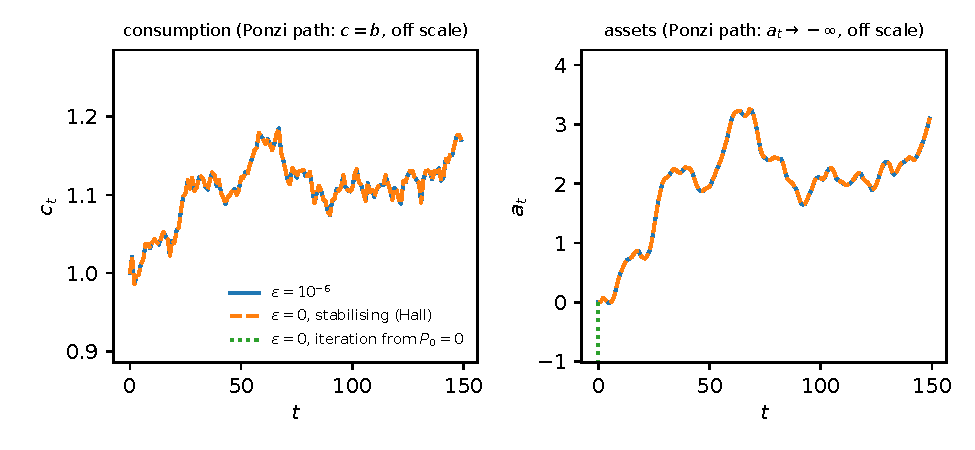
\includegraphics[width=0.95\linewidth]{fig/ls05_pih.pdf}\\[3pt]
\captionof{figure}{Exercise 5.13. Simulated paths with the same shocks. The $\epsilon=10^{-6}$ rule
and Hall's rule overlap; the $\epsilon=0$ iteration limit ($c=b$) leaves the plotted range.}
\end{center}
\end{tcolorbox}

%------- 5.14 -------
\begin{tcolorbox}[evenbox,title={Exercise 5.14 \quad Permanent income model again}]
\begin{tcolorbox}[questionbox]
pp.~154--155. As 5.13 with $y_{t+1}=(1-\rho_1-\rho_2)+\rho_1y_t+\rho_2y_{t-3}+\sigma_y\epsilon_{t+1}$,
initial $a_0,y_0,\dots,y_{-3}$; $\rho_1=.55,\rho_2=.3$, otherwise as 5.13. (a)--(d) as in 5.13.
\end{tcolorbox}

\textbf{Solution:}

\textbf{(a)} The fourth lag forces a longer state: $x_t=[a_t,\ y_t,\ y_{t-1},\ y_{t-2},\ y_{t-3},\ 1]'$,
\[
A=\begin{bmatrix}R&1&0&0&0&0\\0&\rho_1&0&0&\rho_2&1-\rho_1-\rho_2\\0&1&0&0&0&0\\0&0&1&0&0&0\\0&0&0&1&0&0\\0&0&0&0&0&1\end{bmatrix},\quad
B=-e_1,\ C=\sigma_ye_2,
\]
$R_x=\tfrac12\epsilon e_1'e_1+\tfrac12b^2e_6'e_6$, $Q=\tfrac12$, $H=-\tfrac12be_6$; the Bellman
equation is 5.13(a) with $v(a,y_t,y_{t-1},y_{t-2},y_{t-3})$ and next state
$(Ra+y-c,\ y',\ y_t,\ y_{t-1},\ y_{t-2})$.

\textbf{(b)} $\epsilon=10^{-6}$ (772 Riccati steps; DARE agrees):
\[
c_t=0.05265\,a_t+0.21450\,y_t+0.05517\,y_{t-1}+0.05808\,y_{t-2}+0.06113\,y_{t-3}+0.61112,
\]
$d=0.0218$,
with $P_{11}=0.02771$, $P_{22}=0.45999$, $P_{66}=9\,987\,780$ (full $6\times6$ matrix in the notebook).

\textbf{(c)} Eigenvalues of $A-BF$: $0.99998$ (assets), $1$ (constant), and the four roots of
$\lambda^4-0.55\lambda^3-0.3=0$: $0.92682$, $0.12807\pm0.70354i$ ($|\cdot|=0.715$), $-0.63297$ ---
stationary, but with a slow root $0.927$ and an oscillating pair (a four-period pattern).

\textbf{(d)} $\epsilon=0$: the iteration from $P_0=0$ again gives $P=0$, $c_t\equiv b$ (Ponzi). The
stabilising solution is Hall's rule,
$c_t=(1-\beta)[Ra_t+e_1(I-\beta A_y)^{-1}x^y_t]=0.05263a_t+0.21446y_t+0.05516y_{t-1}+0.05806y_{t-2}+0.06112y_{t-3}+0.61120$,
with an exact unit root in assets; the $\epsilon=10^{-6}$ rule is within $8\times10^{-5}$ of it.
Compared with 5.13, the weights on lagged income are all positive: a shock to $y$ comes back via
$\rho_2y_{t-3}$, so older income still carries news about future income, and the permanent-income
annuity $0.05\times E_t\sum\beta^jy_{t+j}$ loads on every lag in the state.
\end{tcolorbox}

%======================================================================
\section*{Companion code}
\addcontentsline{toc}{section}{Companion code}
%======================================================================

Every numerical result above is reproduced by the notebook \texttt{ls\_ch05.ipynb} in this folder
(executed, outputs saved). Each claim is checked by an independent route with an \texttt{assert}.

\begin{center}
\begin{tabular}{@{}lp{11.2cm}@{}}
\toprule
\textbf{Section} & \textbf{What it checks} \\
\midrule
Shared & \texttt{olrp} (5.1(b)), \texttt{dare} (scipy, stabilising), \texttt{howard}, \texttt{evaluate} (Lyapunov). \\
5.1 & Iteration vs DARE vs cross-term removal vs numerical Bellman maximisation. \\
5.2 & Lyapunov vs series vs simulation; monotone $P_j$; Howard vs Riccati; figure. \\
5.3--5.4 & Rules by three routes; Euler-equation residual; impulse responses. \\
5.5--5.6 & Closed form vs Monte Carlo; Lyapunov vs Monte Carlo; finiteness condition. \\
5.7 & Forward program vs closed form vs eigen-decomposition; seigniorage identity; figure. \\
5.8 & LQ vs closed form; invariance to $(w_1,w_2)$; Kalman VAR vs 40-lag OLS; Ponzi limit. \\
5.9 & Certainty equivalence; Kalman log-likelihood vs direct Gaussian density; profile. \\
5.10 & Lyapunov value vs Monte Carlo; Howard limit vs PIH formula. \\
5.11--5.12 & LQ vs Euler closed form; value entries; simulated / Monte Carlo value. \\
5.13--5.14 & $\epsilon>0$ vs DARE; $\epsilon=0$: iteration $\to P=0$, stabilising $=$ Hall. \\
\bottomrule
\end{tabular}
\end{center}

Figures are saved to \texttt{fig/ls05\_*.pdf} with TrueType (not Type~3) fonts.

\end{document}
